\documentclass[11pt]{article}

\usepackage{fullpage}
\usepackage{graphicx}
\usepackage{amsmath}
\usepackage{amssymb}
\usepackage{amsthm}
\usepackage{fancyvrb}

\parindent0in
\pagestyle{plain}
\thispagestyle{plain}

\newcommand{\myname}{Mehshan Mustafa}
\newcommand{\dated}{\today}

\newenvironment{theorem}[2][Theorem]{\begin{trivlist}
\item[\hskip \labelsep {\bfseries #1}\hskip \labelsep {\bfseries #2.}]}{\end{trivlist}}
\newenvironment{lemma}[2][Lemma]{\begin{trivlist}
\item[\hskip \labelsep {\bfseries #1}\hskip \labelsep {\bfseries #2.}]}{\end{trivlist}}
\newenvironment{exercise}[2][Exercise]{\begin{trivlist}
\item[\hskip \labelsep {\bfseries #1}\hskip \labelsep {\bfseries #2.}]}{\end{trivlist}}
\newenvironment{problem}[2][Problem]{\begin{trivlist}
\item[\hskip \labelsep {\bfseries #1}\hskip \labelsep {\bfseries #2.}]}{\end{trivlist}}
\newenvironment{question}[2][Question]{\begin{trivlist}
\item[\hskip \labelsep {\bfseries #1}\hskip \labelsep {\bfseries #2.}]}{\end{trivlist}}
\newenvironment{corollary}[2][Corollary]{\begin{trivlist}
\item[\hskip \labelsep {\bfseries #1}\hskip \labelsep {\bfseries #2.}]}{\end{trivlist}}
\newenvironment{solution}{\begin{proof}[Solution]}{\end{proof}}
\newenvironment{idea}[2][Proof Idea.]{\textit{#1} #2}

\begin{document}

\textbf{Introduction to the Theory of
Computation}\hfill\textbf{\myname}\\[0.01in]
\textbf{Chapter 1: Reqular Languages}\hfill\textbf{\dated}\\
\smallskip\hrule\bigskip

\begin{problem}{1.49 a}
Let $B = \{1^{k}y \ | \ y \in \{0, 1\}^{*} \ and \ y \ contains \ at \ least \ k \ 1s, \ for \ k \geq 1\}$.
Show that $B$ is a regular language.
\end{problem}

\begin{idea}
The regular expression, $1^{k}(0^{*}1)^{k}\{0,1\}^{*}$ describes the language $B_{k}$ for some fixed $k$.
\begin{center}
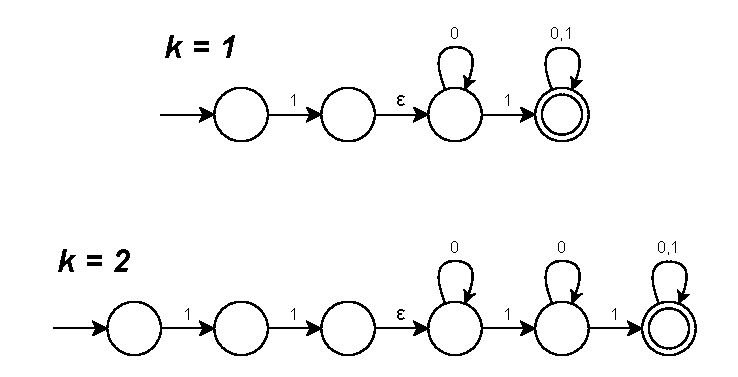
\includegraphics[scale=1.0]{Figures/Problem1.49a.pdf} \\
State diagrams of finite automata that recognize $B_{k=1}$ and $B_{k=2}$.
\end{center}
\end{idea} 

\begin{proof}
\end{proof}

\begin{problem}[Part]{b}
Let $C = \{1^{k}y \ | \ y \in \{0, 1\}^{*} \ and \ y \ contains \ at \ most \ k \ 1s, \ for \ k \geq 1\}$.
Show that $C$ isn’t a regular language.
\end{problem}

\begin{proof}
The proof is by contradiction. Assume $C$ is a regular language. Let $p$ be the pumping lenght given by the puming lemma. Choose $s$ to be the string:
\[ s = 1^{p}01^{p} \]
The string $s$ is a member of $C$, and $|s| \geq p$. Therefore, the pumping lemma guarantees that the string $s$ can be split into three pieces, $s = xyz$, and for each $i \geq 0$ the string $xy^{i}z \in C$. According to the condition 3 $(|xy| \leq p)$, $y$ can only be 1s. But, pumping down the y with $i=0$ results in fewer than $p$ 1s at the start of the string. Thus $xy^{0}z \notin C$, which is a contradiction.
\end{proof}
\end{document}